\chapter{Projektfindung}\label{chp:projektfindung}

    Zu Beginn des Projekts wurden wir von unserem Praxispartner mit drei Fragestellungen konfrontiert, unter denen wir uns für eine wählen konnten:

    \vspace{1em}
    \begin{tabular}{ l|p{13.5cm} }
        \quad & Wie lässt sich der Verkehr für Einkäufe und Lieferungen reduzieren, um die Schadstoffbelastungen in der Luft zu minimieren?
    \end{tabular}
    \\[1em]
    \begin{tabular}{ l|p{13.5cm} }
        \quad & Wie lässt sich die Müllentsorgung in der Innenstadt und in den Grünflächen optimieren (z.B. Roboter, automatische Mülltrennung, Füllstandsensoren etc.)?
    \end{tabular}
    \\[1em]
    \begin{tabular}{ l|p{13.5cm} }
        \quad & Wie lässt sich Informations- und Kommunikationstechnik (IKT) (Rechenzentren, WLAN, Breitband) für eine umwelt- und ressourcenschonende Stadtgestaltung (z.B. Abwärme der Rechenzentren) nutzen? 
    \end{tabular}
    \vspace{1em}

    Im Anschluss des KickOff-Veranstaltung haben wir uns für die zweite Frage, die das Thema Müllentsorgung thematisiert entschieden, da wir dabei die größten Freiheiten bei der Gestaltung des Prototyps gesehen haben und Lust hatten uns mit der Problematik auseinander zu setzen.

    So haben wir in den kommenden Wochen Interviews mit unseren Praxispartnern geführt, nach schon existierende Maßnahmen und der aktuellen Lage vor Ort, sowie nach den psychologischen Gründen recherchiert.
    
    So konnten wir unseren Problemraum immer größer gestalten, bis wir beim CIC Workshop vier Ideen vorgestellt haben. (\href{run:attachments/Frankfurt_Ideen_CIC.pdf}{\textbf{PDF der Präsentation}})

    \begin{figure}[h]
        \begin{center}
            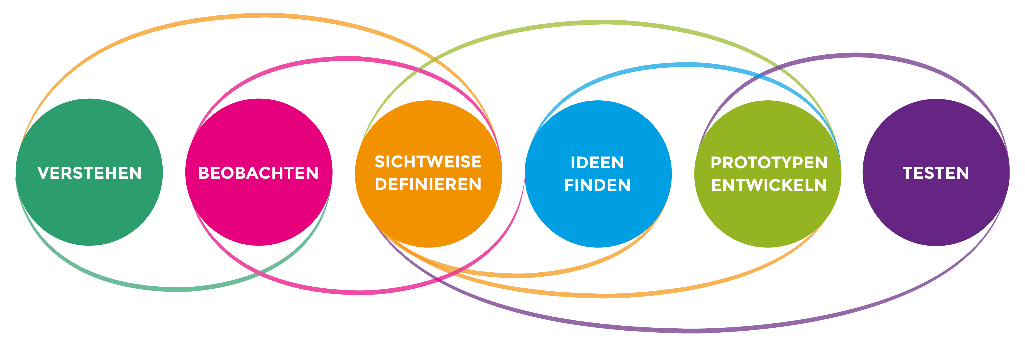
\includegraphics[width=11cm]{media/00_introduction/design_thinking_2.png}
        \end{center}
        \caption{Der Design-Thinking-Prozess\protect\footnote{Quelle: Design Thinking Workshop CrossInnovationClass}}
        \label{fig:dt_2}
    \end{figure}

    \vspace{1em}
    \framebox[\textwidth]{
        \begin{minipage}{\textwidth-1em}
            \vspace{.4em}
            \textbf{Design Thinking}
            \\[1em]            
            Design Thinking ist ein Prozess zur Ideenfindung und -entwicklung.
            Dabei steht der Mensch im Mittelpunkt der mit einem Problem konfrontiert ist.
            
            Abbildung\,\ref{fig:dt_2} zeigt die sechs Phasen die im Prozess durchlaufen werden und visualisiert den iterativen Ansatz, das mehrmalige durchlaufen in unterschiedlichen Kreisen im Laufe des Prozess.\\

            In vielen Veranstaltungen der CIC ist uns besonders das Modell des \enquote{Double Diamonds} (Abbildung\,\ref{fig:dt_1}) begegnet, da der Ablauf der Cross in einem solchen Rahmen strukturiert wurde.
            Anhand der Fragestellung wird ein breiter Problemraum geöffnet in dem möglichst viel Wissen aus verschiedenen Perspektiven zusammenfließt. Diese Problemdefinition wird nun konkretisiert, um einen Lösungsraum zu öffnen, der Lösungsansätze jeder Art zulässt.
            Anschließend werden auch diese im Team besprochen und am Ende entsteht ein konkreter Prototyp.
            \vspace{.4em}
        \end{minipage}
    }
    \vspace{1em}

    \begin{figure}[h]
        \begin{center}
            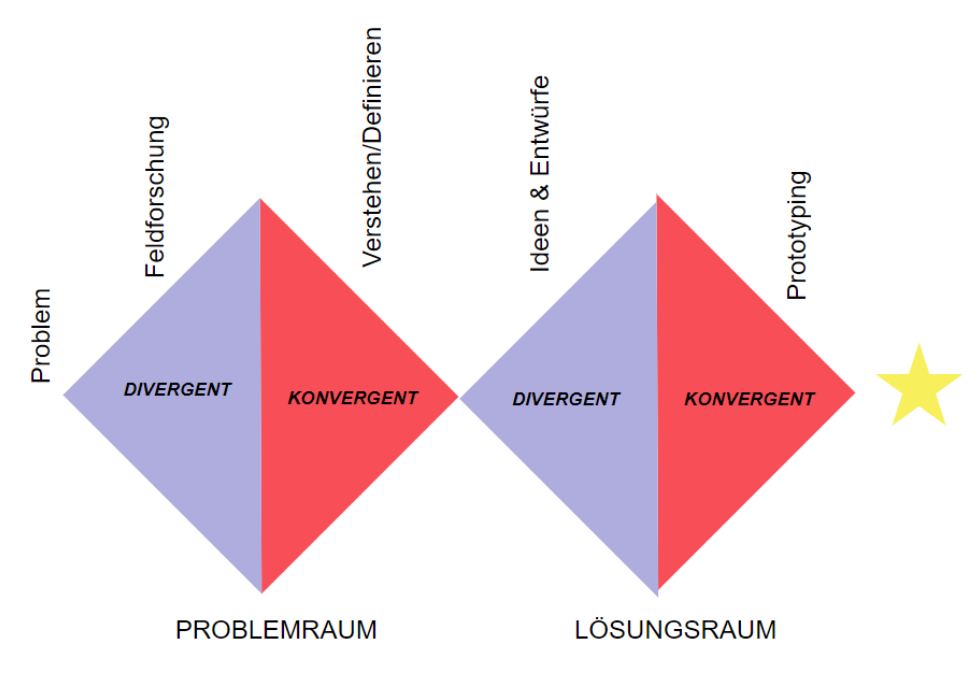
\includegraphics[width=10cm]{media/00_introduction/design_thinking_1.png}
        \end{center}
        \caption{Denkmodell \enquote{Double Diamond}\protect\footnotemark[\value{footnote}]}
        \label{fig:dt_1}
    \end{figure}

    Dabei hatten wir zwei Favoriten.

    Die Idee, die es nicht geschafft hat, war der sogenannte \enquote{Bar-Bus}.Er sollte ein ausgebauter Bully sein, der verschiedene Konzepte vereint hätte. Darunter fällt ein  als Rutsche umgesetzter Flascheneinwurf, die Möglichkeit den Bus zu beschreiben und bemalen, sowie ein Angebot Snacks in müllfreier Verpackung und Entertainment-Angebote, wie Musik.
    Er sollte eine Anlaufstelle für die Menschen werden, die Aufgrund ihrer Kleidung, ihres Ausshehens oder ihrer finanziellen Mittel oft den Zugang  zu den Frankfurter Clubs verwehrt bekommen.

    Problematisch an der Idee war, dass die Stadt hier als Anbieter von Waren auftritt und ebenfalls die Party-Stimmung nicht mindert, auch wenn dadurch wohlmöglich die aggressive und rücksichtslose Atmosphäre minimiert wird.

    Daher haben wir im weiteren Verlauf unsere zweite Idee, einen interaktiven Mülleimer verfolgt, den wir im nächsten Kapitel ausführlich beschreiben.


\chapter{Projektbeschreibung}

\section{Integrierte Konzepte}
    
    Die Idee des Licht-Mülleimers (anfänglich auch als \enquote{Party-Bin} bezeichnet) soll das Problem lösen, dass manche Feiernden den Weg zum Mülleimer nicht finden, sodass, vorallem in der Corona-Zeit, die Parks und Plätze sowie das Main-Ufer Samstag und Sonntag Morgens extrem vermüllt waren.

    Den ersten psychologischen Effekt den wir auf unsere Seite holen wollten, ist ein Aspekt der Gamification. Wir wollten die Menschen belohnen dafür, dass sie den Mülleimer verwendet haben. Dabei wollten wir erreichen dass der Mülleimer selbst auf den Mülleinwurf reagiert.Dabei war uns wichtig, dass es einfach und intuitiv bleibt, keine App, kein komplexes Konzept, ein einfaches Feedback, das jeden Mülleinwurf belohnt.

    Die möglichen Feedbackansätze bestanden in unseren Überlegungen aus einem auditiven Feedback, bspw. einem Geräusch, einer menschlichen Stimme oder  Musik oder einem visuellem Feedback, welches per direkter oder indirekter Beleuchtung zu realisieren wäre.

    In unserem ersten Ansatz haben wir uns auf Musik fokussiert, die Möglichkeit belohnt zu werden in dem man beim Einwurf für ein nächstes Lied abstimmen kann, oder als Ansatz um die Feiernden in die Nähe der Mülleimer zu bekommen, eine Abstimmung an der jeder Mülleimer ein Lied repräsentiert und misst, wieviele Menschen um ihn herrum stehen. Bei diesem Ansatz konnten wir ein paar große Risiken nicht ausmerzen, einerseits ebenfalls das Argument, dass diese Mülleimer die Partystimmung stärker anheizen könnten, andererseits das Thema der Rechte an der Musik.
    Ein Beispielentwurf ist in der Skizze\,\ref{fig:standing_desk_bin_1} zu sehen.

    \begin{figure}[H]
        \centering
        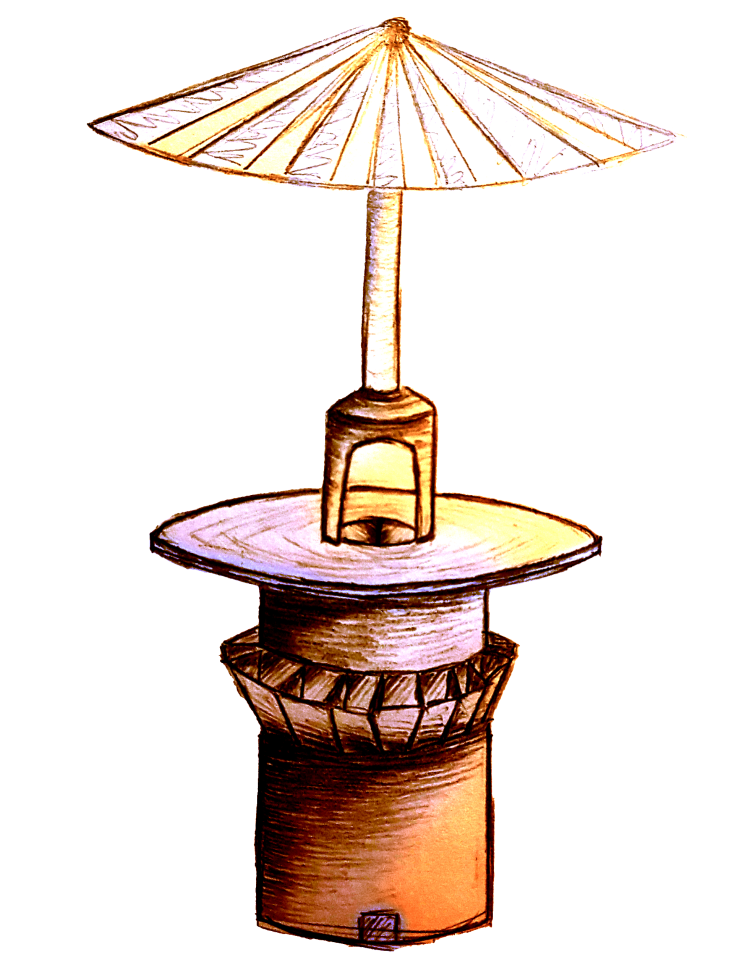
\includegraphics[width=5cm]{media/01_project/sketch_standing_table_bin.png}
        \caption{Konzept eines Tischmülleimers, der einige der Konzepte umsetzt.}
        \label{fig:standing_desk_bin_1}
    \end{figure}

    Der zweite Ansatz beruht nun stärker auf dem Licht-Aspekt.
    Ein erster Entwurf des ganzen ist die Skizze\,\ref{fig:light_bin_1}
    Dieser Mülleimer reagiert beim Einwurf von Müll mit einer kleinen \enquote{Lichtshow}\\

    In beiden Skizzen (\ref{fig:standing_desk_bin_1} \& \ref{fig:light_bin_1}) zu entdecken ist ein Pfandring. Da bei unseren Recherchen rauskam, dass ein großer Teil des anfallenden Mülls auf intakte wie zerschlagene Flaschen zurückzuführen ist und wir von Jochen Schmitz eine positive Erfahrung mit einem sogenannten \enquote{Pfandregal} geschildert bekommen haben, wollten wir einen Flaschenring in unser Design integrieren.   



    \begin{figure}[H]
        \centering
        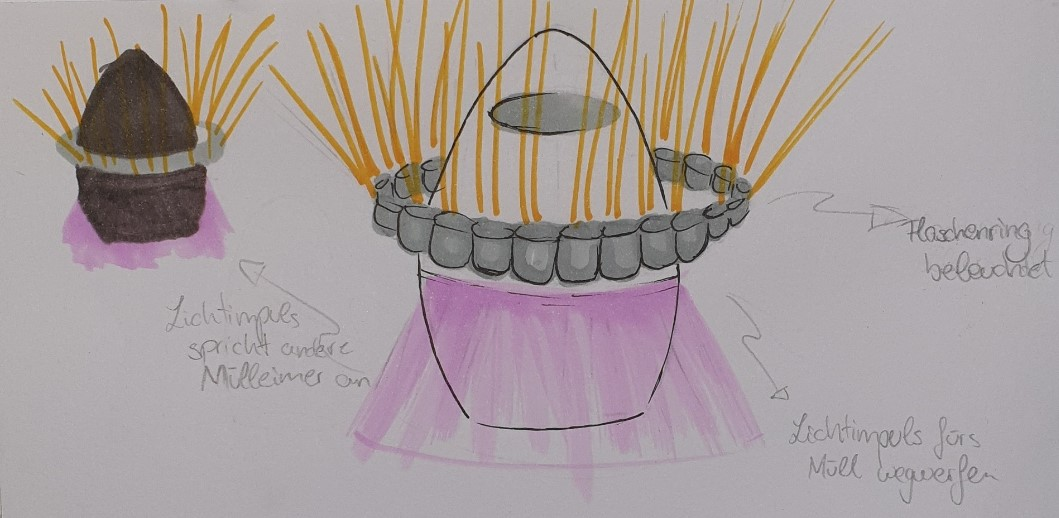
\includegraphics[width=10cm]{media/01_project/sketch_party_bin.jpg}
        \caption{Konzept eines Tischmülleimers, der einige der Konzepte umsetzt.}
        \label{fig:light_bin_1}
    \end{figure}

    Ausgehend aus diesen Überlegungen haben wir letztendlich ein finalen Entwurf zusammengestellt. Dieser ist minimalistischer im Design und in der Art der Beleuchtung, um sich besser ins Stadtbild einzufügen.


    \begin{figure}[H]
        \centering
        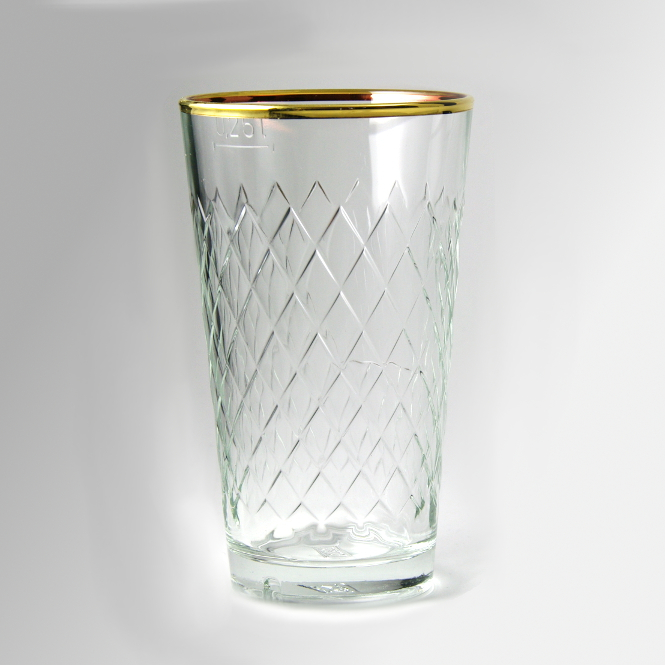
\includegraphics[width=5cm]{media/01_project/picture_geripptes.jpg}
        \caption{Das \enquote{Gerippte}.}
        \label{fig:picture_gerippte}
    \end{figure}


    Das finale  Design entleiht sich die Rauten am Rand vom in Frankfurt wohlbekannten Kulturgut: Das Gerippte, ein Apfelwein Glas das sich hoher lokaler Beliebtheit  erfreut. Ein Beispielglas ist in der Abbildung\,\ref{fig:picture_gerippte} zu sehen.

    Eingehendere Beschreibung der Projekt-Idee untermauert mit
    Skizzen/Zeichnungen
    
    \begin{figure}[H]
        \centering
        \begin{subfigure}[b]{\textwidth}
            \centering
            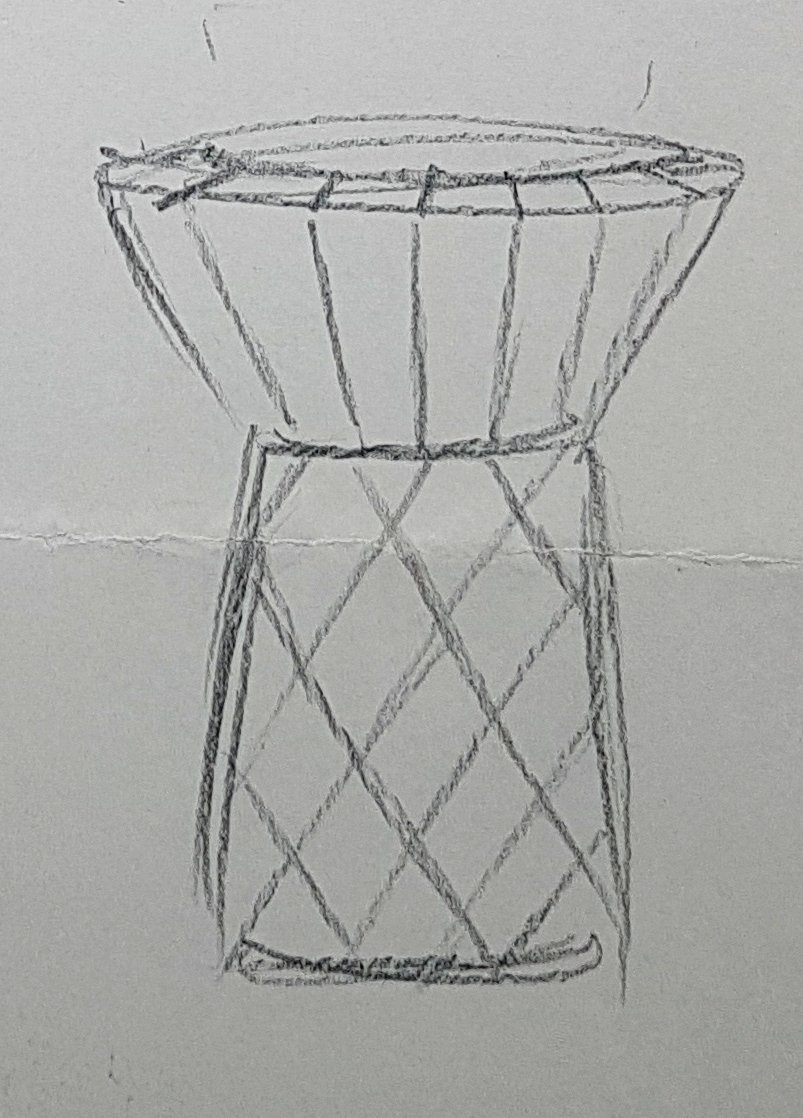
\includegraphics[width=0.32\linewidth]{media/01_project/pencil_sketch_bin_2.jpg}
            \hspace{1cm}
            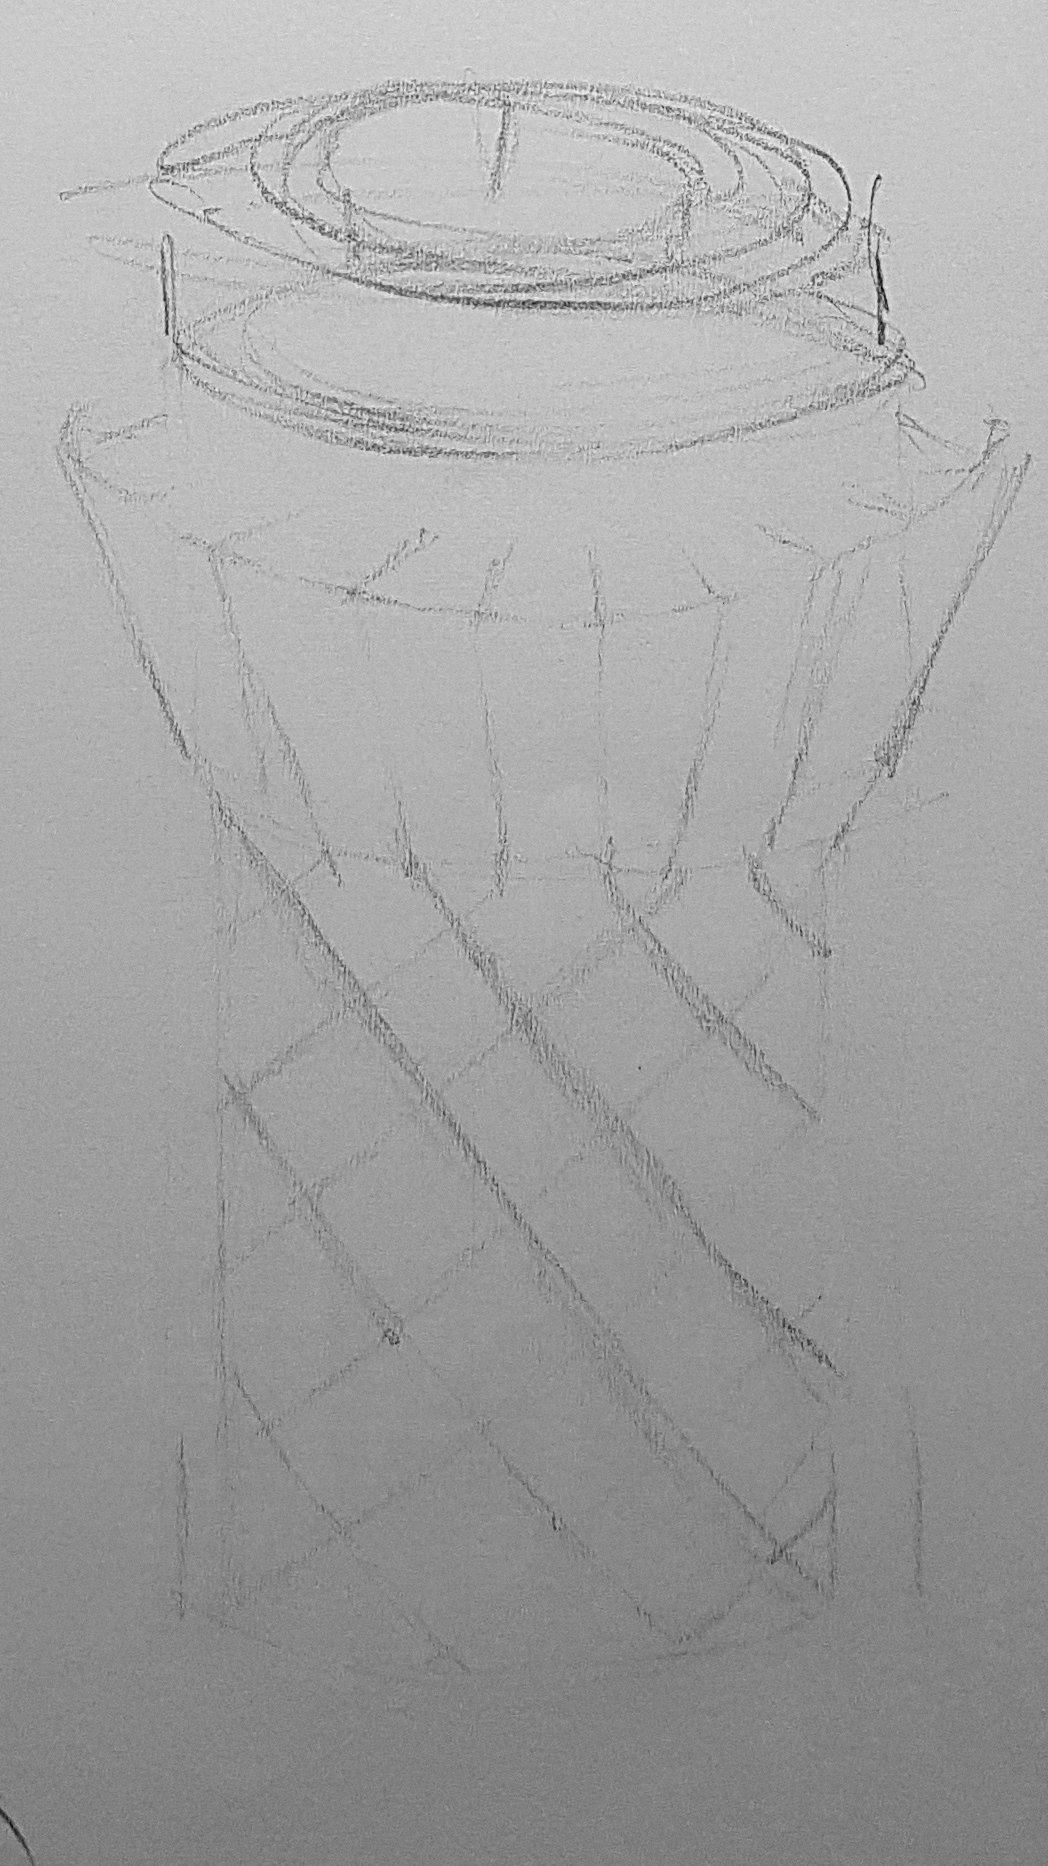
\includegraphics[width=0.32\linewidth]{media/01_project/pencil_sketch_bin_3.jpg}
        \end{subfigure}
        \caption{Skizze des Entwurfs mit Rautenmuster}
        \label{fig:pencil_bin_2}
    \end{figure}

    \begin{figure}[H]
        \begin{center}
            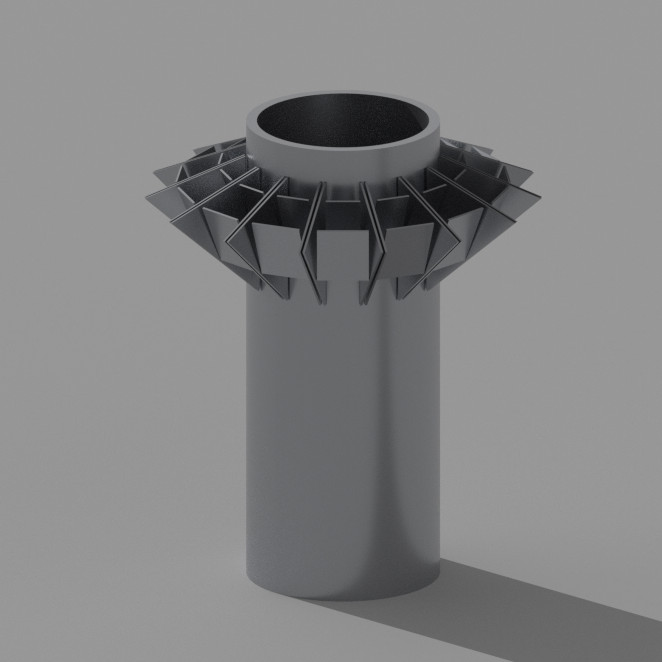
\includegraphics[width=7cm]{media/01_project/render_bin.jpg}
        \end{center}
        \caption{Render des Entwurfs mit Fokus auf den Flaschenring}
        \label{fig:pencil_bin_3}
    \end{figure}

\section{Funkionen}

    Der Gerippte, so wurde er nun getauft, besitzt folgende Funktionen:


